\documentclass[12pt]{ctexart} % 使用 ctexart 文档类支持中文

\usepackage{fancyhdr} % 奇特的 header
\usepackage{xcolor} % 更多颜色

\usepackage[utf8]{inputenc} % 支持 UTF8 字符,在 UTF8 engine 中无需此行
\usepackage{xeCJK} % 支持中文排版,已经包含在 ctexart 中
\usepackage{fontspec} % 字体设置
\usepackage{geometry} % 页面布局
\usepackage{titlesec} % 自定义标题样式
\usepackage{setspace} % 设置行距
\usepackage{microtype} % 更多的微调
\usepackage{tabularx} % 表格支持

\usepackage{float} % Add the float package,支持图片位置固定

\usepackage[colorlinks,linkcolor=black,urlcolor=black]{hyperref} % 超链接支持

\usepackage{tocloft} % 自定义目录样式

\usepackage{graphicx} % 图片设置
\graphicspath{ {./images/} }

% 设置页面布局
\geometry{a4paper, margin=1in}

% 设置行距为 1.25 倍
\setstretch{1.25}

% 设置中文字体
\setCJKmainfont{SimSun}[BoldFont={Microsoft YaHei Bold}] % 设置正文为宋体

\setCJKsansfont{Microsoft YaHei}[BoldFont={Microsoft YaHei Bold}] % 标题等无衬线字体为黑体

% 设置英文字体
\setmainfont{Times New Roman}



% 配置页眉和页脚
\pagestyle{fancy}
\fancyhf{}
\renewcommand{\headrulewidth}{0pt}

\setlength{\headheight}{25.60938pt} % Set the headheight to the required value
\addtolength{\topmargin}{-13.60938pt} % Adjust the topmargin to compensate

% 定义颜色
\definecolor{myblue}{RGB}{152, 220, 222} % 蓝色

% 左侧页眉设置, 页码在页眉外侧
\fancyhead[L]{%
  \colorbox{myblue}{%
    \parbox[t]{1cm}{%
      \textcolor{white}{\thepage}%
    }%
  }%
  \hspace{0.5cm}
  软件需求规格说明书
}

% \fancyhead[L]{\leftmark} % 左页显示章节名

% 页眉横线设置
\renewcommand{\headrulewidth}{0.5pt}
\renewcommand{\headrule}{%
  \hbox to\headwidth{%
    \color{black}\leaders\hrule height \headrulewidth\hfill%
  }%
}


% 设置目录样式
\renewcommand{\cftsecfont}{\bfseries} % 目录中章节标题加粗

\titleformat{\section}
  {\normalfont\Large\bfseries} % 移除 \centering
  {\thesection}{1em}{}


% 超链接设置
\hypersetup{
  colorlinks=true,
  linkcolor=black,
  filecolor=magenta,      
  urlcolor=cyan,
}


\begin{document}

\begin{titlepage}
  \centering % 居中对齐
  \vspace*{2cm} % 从顶部添加一些垂直间距
  
\includegraphics[width=0.6\textwidth]{zjutitle.jpg} % 插入图片
  
  \vspace{2cm} % 添加垂直间距
  
  {\fontsize{36}{48}\selectfont\CJKfontspec{Microsoft YaHei} 软件需求规格说明书} % 标题
  
  \vspace{2cm} % 添加垂直间距
  
  
\includegraphics[width=0.4\textwidth]{zjulogo.jpg} % 插入图片
  
  \vspace{2cm}
  
  {\Huge\CJKfontspec{Microsoft YaHei}  项目主题:H5游戏分享平台} % 项目主题
  
  \vspace{1cm}

  {\Large\CJKfontspec{Microsoft YaHei} 小组成员:} % 作者
  
  \vspace{1cm} % 添加垂直间距
  
  {\Large\CJKfontspec{Microsoft YaHei} \today} % 日期

\end{titlepage}

\newpage
\tableofcontents % 自动生成目录
\newpage

\section{引言}

\subsection{编写目的}
该项目的目的是实现一个HTML5游戏分享平台,用于游戏分享、展示和交流。

此软件需求规格说明书描述该项目功能性需求和非功能性需求,详细描述软件的功能、性能、约束条件等,确保相关方对需求有统一理解。
此文档旨在为开发人员提供开发过程的参照,为开发团队提供清晰的开发依据,使开发人员能明确任务以及期限,确保软件按预期设计和实现。
同时也为测试和验收提供标准,确保软件满足需求,并为后续维护提供参考。

\subsection{项目背景}
该项目开发的软件为一个HTML5游戏分享平台。
随着互联网技术的发展,HTML5技术凭借其跨平台兼容性、无需插件加载、即点即玩的特性,已成为游戏开发与传播的重要载体。
传统游戏平台更多面向客户端或主机游戏,而轻量化、低门槛的HTML5游戏往往分散于各类网站或社交媒体中,缺乏统一的展示、体验与互动空间。
在此背景下,构建一个专注于HTML5游戏的在线分享平台,既是技术发展的必然趋势,也是满足用户需求的关键举措。

相较于传统游戏分发模式,HTML5游戏分享平台让玩家随时随地通过浏览器畅玩游戏,同时为开发者提供低成本、高效率的作品展示渠道。
对玩家而言,平台可汇聚海量创意游戏,通过标签分类、用户评分与社区推荐快速发现优质内容;
对开发者而言,平台既能成为技术交流的窗口,又能通过用户反馈优化作品,甚至实现商业化潜力;
此外,随着教育领域对编程与游戏化教学需求的增长,该平台还可作为教学案例库,助力游戏爱好者学习游戏开发技术。

在互联网时代,游戏行业的技术风向与用户偏好瞬息万变,而游戏社区就是游戏发展壮大的土壤,是游戏不断进步的根基。
HTML5游戏分享平台能够构建动态交互社区生态:玩家可实时分享攻略、录制精彩片段;开发者能发布技术日志、参与话题讨论;
平台也会进行数据分析,为游戏优化提供依据。最终能形成“创作-体验-反馈”的良性循环。


\subsection{名词定义}
HTML5:超文本标记语言第五版(Hypertext Markup Language 5),是HTML的最新演进标准,支持多媒体、图形和动画的直接嵌入,无需依赖第三方插件(如Flash)。
它是构建现代网页及浏览器端游戏的核心技术,具备跨平台兼容性,适用于PC、移动设备等多种终端。

CSS:层叠样式表(Cascading Style Sheets),是一种用来表现 HTML 等文件样式的计算机语言,在网页中能够对网页中元素位置的排版进行像素级精确控制。

JavaScript:一种直译式脚本语言,其引擎是现代浏览器的一部分,可以用来给网页增加动态功能。

Next.js:一个基于React的开源JavaScript框架,提供了服务器端渲染、内容动态生成、增量生成页面等核心功能来简化开发流程并优化性能。

DBMS:数据库管理系统(Database Management System),是由数据库及其管理软件组成的集可运行的存储、维护和应用系统提供数据为一体的软件系统。

CMS:内容管理系统(Content Management System),是一种用于创建、编辑、管理和发布数字内容的软件平台。
它允许用户通过直观的界面管理网站内容,而无需编写代码或具备专业技术知识。
CMS通常支持多用户协作、版本控制、权限管理等功能,广泛应用于在线社区等领域。

\section{总体描述}
\subsection{产品前景}
该项目开发的网站是一个HTML5游戏分享平台,用于游戏分享、展示和交流。
开发者可以发布游戏,优化更新;玩家可以在线游玩,发表评论。

随着HTML5技术的成熟与跨平台特性的普及,互联网已成为游戏创新与传播的重要载体。HTML5游戏无需依赖复杂安装、适配多终端的特点,正逐步改变传统游戏分发模式。
本平台旨在构建一个开放的在线游戏分享生态,为开发者提供便捷的作品发布渠道,同时让玩家通过浏览器即可即时体验轻量化游戏。
在数字化娱乐需求日益增长的背景下,用户对快速获取优质游戏内容的需求愈发迫切。
与传统游戏依赖下载安装的分发方式相比,本平台通过“即点即玩”的特性大幅降低游戏试玩门槛,促进创作者与玩家的直接互动,
推动独立游戏社区发展,并为中小型开发者提供更多曝光机会,从而激发游戏行业的创新活力。
这一模式既是游戏行业去中心化趋势的体现,也是互联网技术赋能创意经济的重要实践,未来将助力构建更开放、包容的游戏生态系统。

\subsection{用户类及其特征}
实际产品进行了交付后的产品使用方拥有三种角色,我们将其定义为三个用户类,分别为管理员、普通用户、游客。如图一所示。

\begin{figure}[htbp]
  \centering
  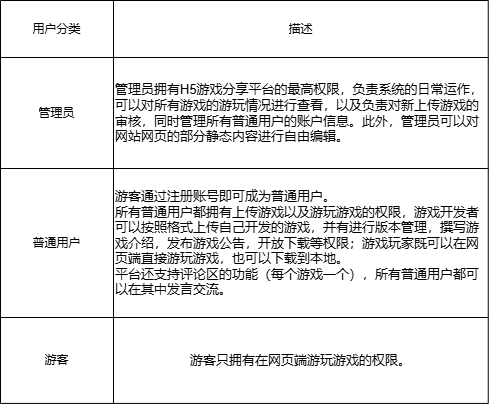
\includegraphics[width=0.8\textwidth]{user_class.png}
  \caption{用户类}
  \label{f1}
\end{figure}


\subsection{产品功能}
产品使用者可分为上述的三种用户,依照各个用户所拥有的权限,H5游戏分享平台的功能如图二所示。

\begin{figure}[htbp]
  \centering
  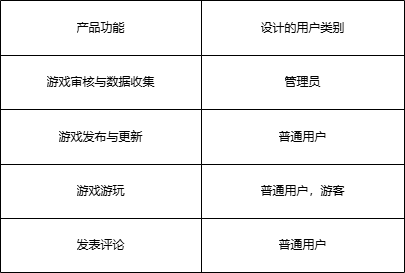
\includegraphics[width=0.8\textwidth]{function.png}
  \caption{产品功能}
  \label{f2}
\end{figure}

\subsection{运行环境}
H5游戏分享平台网站需要通过现代网页浏览器进行访问及操作,较新的浏览器版本可以获得更好的体验。

\subsection{设计和实现上的约束}
系统的设计、编码以及维护将遵照后续提交的《项目总体计划》等文档中的具体要求进行。

在具体设计和实现上,按照以下约束进行:

(1)数据存储

平台采用 drawdb 数据库作为核心数据存储引擎,用于管理用户信息、游戏元数据、评论及交互记录等结构化数据。
数据库设计需满足第三范式(3NF),确保数据一致性和可维护性。

(2)网络服务性能

平台需支持至少100名用户同时在线,并在高峰时段保证核心接口(如游戏加载、用户登录、数据提交)的响应时间不超过1s。

(3)数据安全

完整性保障:
用户上传的游戏文件需要加密,防止在未经授权的情况下被篡改,关键数据的传输可能需要加密。

保密性要求:
用户敏感信息需要加密存储,加密技术必须自动,实时,精确,可靠。可能需要实现安全的第三方登录授权。

可用性限制:
需要通过对使用者的身份验证来防止越权操作,并为合法使用者提供安全便捷的使用。

(4)跨平台兼容性

平台需要兼容主流浏览器的最新版本,并确保HTML5游戏在PC端和移动端的渲染一致性。



\subsection{用户文档}
平台交付时将提供三类用户文档:描述类文档、过程类文档、参考类文档,
旨在帮助用户快速熟悉平台功能,并通过文档高效解决使用中的问题。

(1)描述类文档

描述类文档提供对HTML5游戏分享平台的核心功能、系统架构、界面设计、用户权限及交互特性的全面说明,包括
网站的核心模块(如游戏库、评论区)及其用途,游戏上传/下载、在线试玩、用户评论等功能的具体描述。

(2)过程类文档

过程类文档通过交互式引导和分步教程帮助用户完成关键操作,包括
注册/登录流程等新用户引导,游戏上传/试玩/社交互动等核心功能指引,以及对开发者工具如何使用的提示。

(3)参考类文档

参考类文档按功能模块和常见问题分类,提供精准解决方案,包括了
问题排查指南,网站功能详解,开发者文档,隐私与安全建议。
为用户提供问题的快速解决方案,以便于用户进行操作。


\section{系统功能}
\subsection{用户需求}
% 在这里添加用户需求的内容
本节根据用户提出的需求描述系统的功能,首先列出各类用户的需求。

游客:

\begin{tabular}{|c|c|c|}
  \hline
  序号& 优先级& 需求内容\\
  \hline
  1 & 高& 在线游玩游戏\\
  \hline
\end{tabular}

\vspace{1cm}
普通用户:

\begin{tabular}{|c|c|c|}
  \hline
  序号& 优先级& 需求内容\\
  \hline
  1 & 高& 上传游戏,填写元数据:标题、描述、分类标签、缩略图\\
  \hline
  2 & 高& 管理自己上传的游戏,支持更改游戏,下架游戏等\\
  \hline
  3 & 中& 收藏心仪的游戏,方便之后游玩\\
  \hline
  4 & 中& 分类浏览,按标签(如“休闲”“策略”)筛选游戏\\
  \hline
  5 & 低& 评论区,为用户提供交流功能\\
  \hline
  6 & 低& 给游戏评分,查看游戏评分\\
  \hline
  7 & 高& 下载游戏,提供游戏包下载链接\\
  \hline
\end{tabular}

\vspace{1cm}
平台管理员:

\begin{tabular}{|c|c|c|}
  \hline
  序号& 优先级& 需求内容\\
  \hline
  1 & 高& 审核新游戏(内容合规性等)\\
  \hline
  2 & 中& 违规游戏下架并通知开发者\\
  \hline
  3 & 低& 维护游戏分类标签\\
  \hline
\end{tabular}

\subsection{用例图}

图 \ref{fig:all-use-case-brief} 展示了系统大致的用例图以及和第三方媒介的交互;图 \ref{fig:all-use-case-unorg} ,以不同用户分类的方式展示了系统更加细致的用例。

\begin{figure}[htbp]
  \centering
  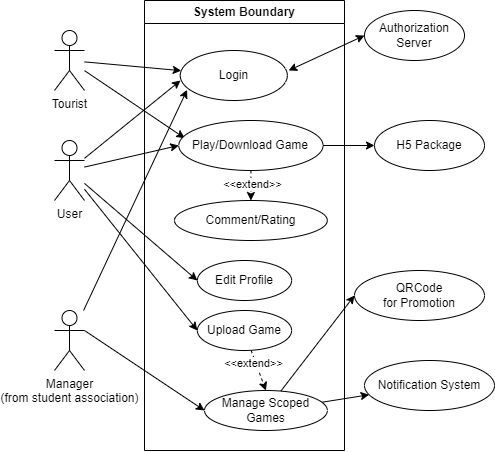
\includegraphics[width=0.6\textwidth]{all_use_case.png}
  \caption{粒度精简用例图}
  \label{fig:all-use-case-brief}
\end{figure}

\begin{figure}[htbp]
  \centering
  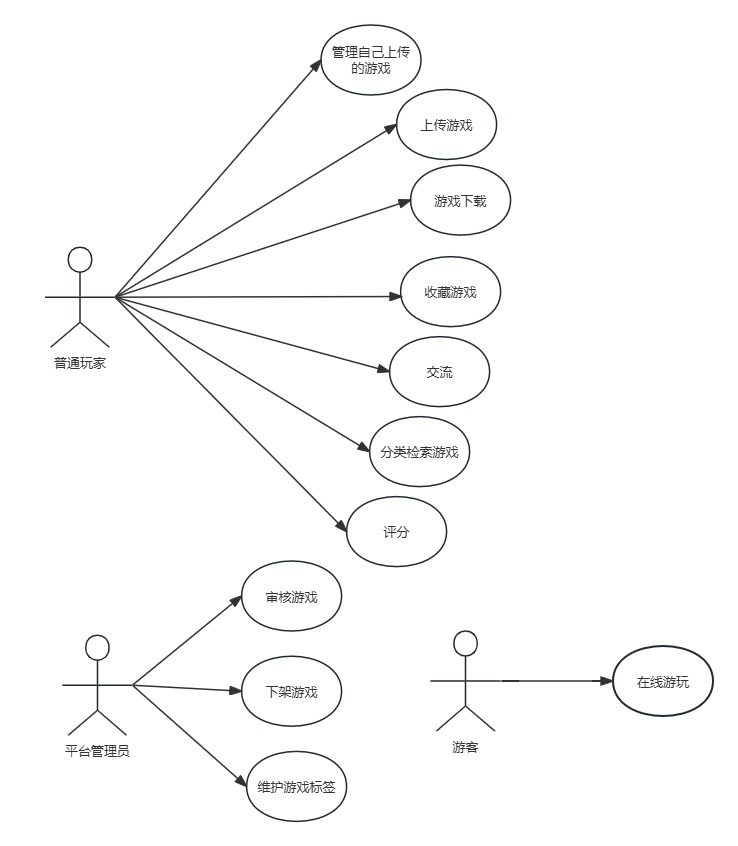
\includegraphics[width=0.6\textwidth]{yongli.jpg}
  \caption{粒度优化用例图}
  \label{fig:all-use-case-unorg}
\end{figure}

\subsection{功能列表}
\subsubsection{注册}
用户开始需要注册符号自己的账号,,初始管理员在系统部署阶段生成。
用户登录系统应该能根据用户输入的账户与密码验证其合法性。注册成功后系统返回登录界面。

主要流程请求/响应时序图:

\begin{figure}[htbp]
  \centering
  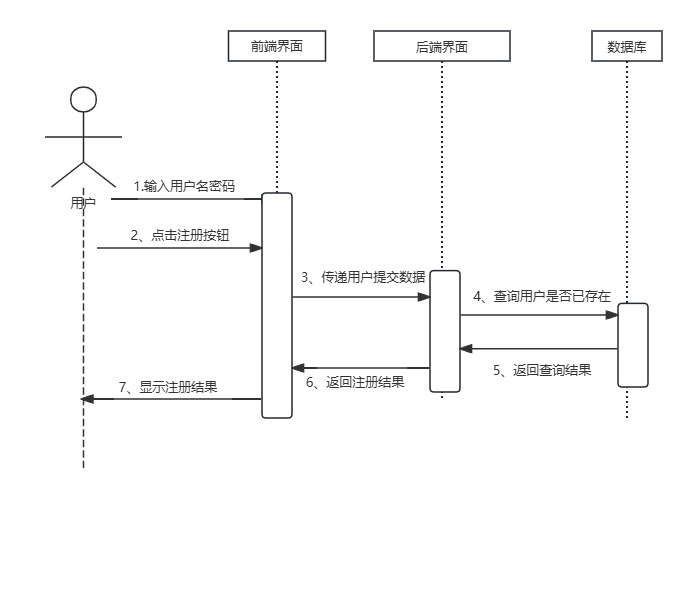
\includegraphics[width=0.8\textwidth]{yongli1.jpg}
  \caption{注册主要流程请求/响应时序图}
\end{figure}

用例文档:

\begin{tabular}{|c|c|}
  \hline
  用例名称& 用户注册\\
  \hline
  用例编号 & USE-CASE-1\\
  \hline
  行为角色 & 普通用户\\
  \hline
  简要说明 & 用户应能够注册以拥有自己的账号\\
  \hline
  优先级 & 高\\
  \hline
  前置条件 & 进入注册界面\\
  \hline
  后置条件 & 注册完成后返回登录界面\\
  \hline
  流程 & 1、用户打开登录界面\\
      & 2、用户输入账号密码\\
      & 3、用户点击注册按钮提交\\
      & 4、如果注册成功,显示失败提示信息,回到第 2 步\\
      & 5、注册成功系统返回登录界面\\
  \hline
  异常处理 & 无论注册失败或成功,以弹窗的方式显示反馈信息\\
  \hline
  备注 & 无\\
  \hline
\end{tabular}

\subsubsection{登录}
普通用户在使用系统前必须进行登录。注意为了安全性,如 \ref{fig:login-sequence} 流程图这样的自建鉴权系统仅供参考。真正开发部署时将采样更简易安全的 OAuth2.0 第三方登录系统。

主要流程请求/响应时序图:

\begin{figure}[ht]
  \centering
  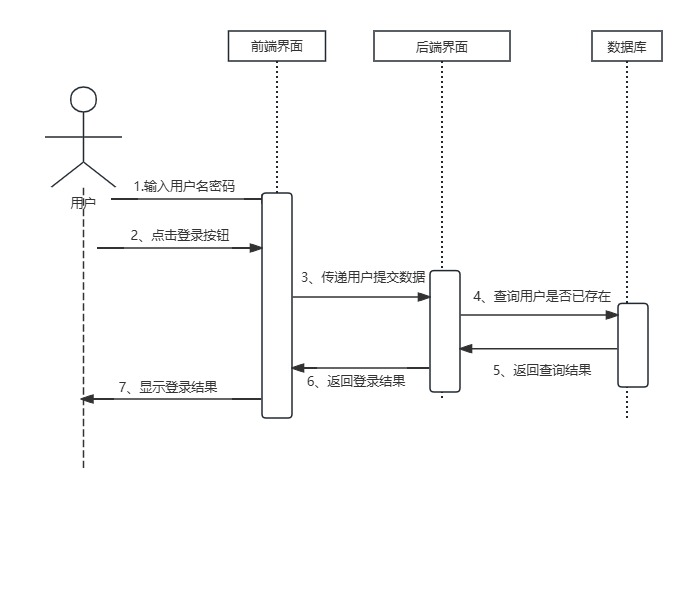
\includegraphics[width=0.8\textwidth]{yongli2.jpg}
  \caption{登录主要流程请求/响应时序图}
  \label{fig:login-sequence} % 为图片添加标签
\end{figure}

用例文档:

\begin{tabular}{|c|c|}
  \hline
  用例名称& 用户登录\\
  \hline
  用例编号 & USE-CASE-2\\
  \hline
  行为角色 & 普通用户,平台管理员\\
  \hline
  简要说明 & 用户应能登录自己的账号\\
  \hline
  优先级 & 高\\
  \hline
  前置条件 & 进入登录界面\\
  \hline
  后置条件 & 登录成功后进入平台首页\\
  \hline
  流程 & 1、用户进入登录界面\\
      & 2、 输入账号密码\\
      & 3、点击登录提交信息\\
      & 4、成功则进入首页\\
      & 5、失败提示错误返回登录界面\\
  \hline
  异常处理 & 无论登录失败或成功,以弹窗的方式显示反馈信息\\
  \hline
  备注 & 无\\
  \hline
\end{tabular}

\subsubsection{登出}
用户在登录之后可以选择登出,该操作让用户退出登录状态。登出成功后系统将返回到登陆界面

主要流程请求/响应时序图:
\begin{figure}[ht]
  \centering
  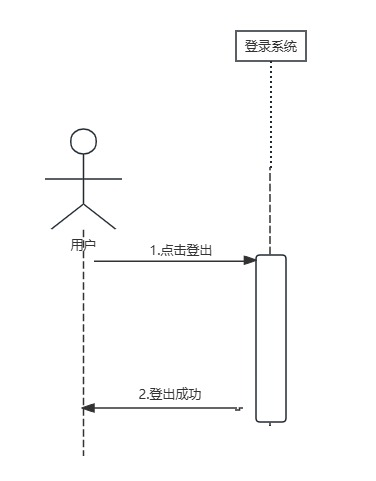
\includegraphics[width=0.5\textwidth]{yongli3.jpg}
  \caption{登出主要流程请求/响应时序图}
\end{figure}
用例文档:

\begin{tabular}{|c|c|}
  \hline
  用例名称& 用户登出\\
  \hline
  用例编号 & USE-CASE-3\\
  \hline
  行为角色 & 普通用户,平台管理员\\
  \hline
  简要说明 & 用户应能登出自己的账号\\
  \hline
  优先级 & 高\\
  \hline
  前置条件 & 已登录状态\\
  \hline
  后置条件 & 返回登录界面\\
  \hline
  流程 & 1、点击登出按键\\
      & 2、返回登录界面\\
  \hline
  异常处理 & 无\\
  \hline
  备注 & 无\\
  \hline
\end{tabular}

\subsubsection{在线游玩与下载}
用户可以在游戏浏览界面或者自己的游戏收藏界面点击心仪的游戏进入该游戏界面,
该界面下包括游戏的信息:标题、描述登;同时支持在线游玩与下载

主要流程请求/响应时序图:
\begin{figure}[ht]
  \centering
  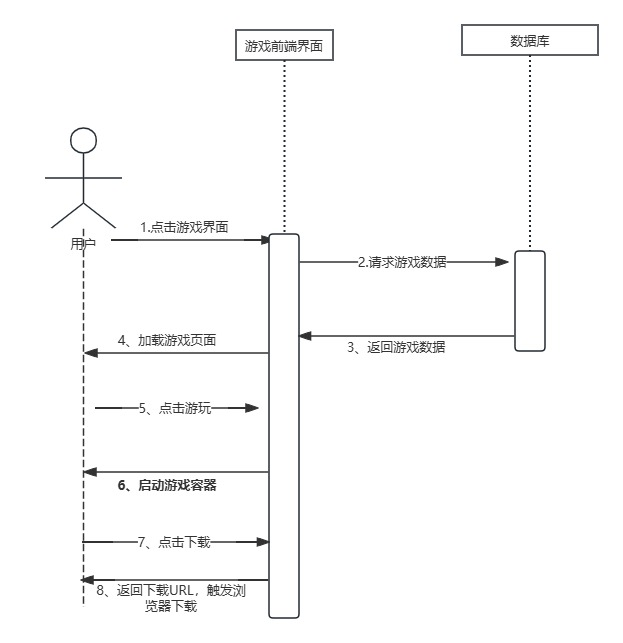
\includegraphics[width=0.7\textwidth]{yongli4.jpg}
  \caption{在线游玩与下载主要流程请求/响应时序图}
\end{figure}
用例文档:

\begin{tabular}{|c|c|}
  \hline
  用例名称& 在线游玩与下载\\
  \hline
  用例编号 & USE-CASE-4\\
  \hline
  行为角色 & 普通玩家,游客\\
  \hline
  简要说明 & 用户应能在线游玩与下载平台上的游戏\\
  \hline
  优先级 & 高\\
  \hline
  前置条件 & 已登录\\
  \hline
  后置条件 & 无\\
  \hline
  流程 & 1、点击游戏进入该游戏界面\\
      &  2、等待游戏加载完毕\\
      & 3、点击开始游玩开始在线游玩\\
      & 4、点击下载按钮下载游戏\\
  \hline
  异常处理 & 无\\
  \hline
  备注 & 游客仅可在线游玩,\\
       &需要保证用户的在线游玩的流畅体验以及游戏下载速度\\
  \hline
\end{tabular}

\subsubsection{分类浏览游戏}
支持用户通过在浏览界面选中游戏分类标签以呈现带有这些游戏标签的游戏,方便用户检索到自己心仪的游戏
这些标签选项由平台给出,游戏创作者在上传游戏时为自己的游戏选中对应的标签。

主要流程请求/响应时序图:
\begin{figure}[ht]
  \centering
  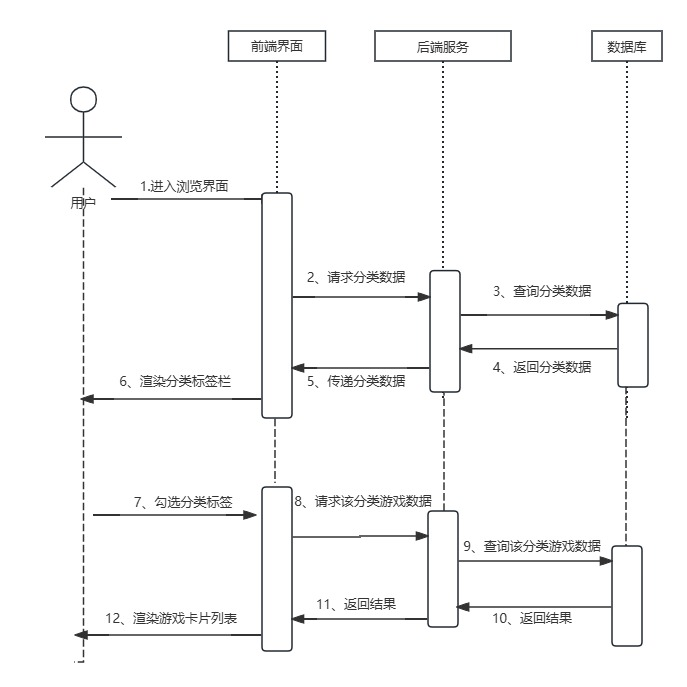
\includegraphics[width=0.6\textwidth]{yongli5.jpg}
  \caption{分类浏览主要流程请求/响应时序图}
\end{figure}
用例文档:

\begin{tabular}{|c|c|}
  \hline
  用例名称& 分类浏览游戏\\
  \hline
  用例编号 & USE-CASE-5\\
  \hline
  行为角色 & 普通用户,游客\\
  \hline
  简要说明 & 用户应能分类检索游戏\\
  \hline
  优先级 & 低\\
  \hline
  前置条件 & 已登录\\
  \hline
  后置条件 & 呈现带有这些标签的游戏\\
  \hline
  流程 & 1、进入游戏浏览界面\\
       & 2、选中标签\\
       & 3、点击确认\\
       & 4、等待网页重新加载完毕开始浏览\\
  \hline
  异常处理 & 无\\
  \hline
  备注 & 需要保证系统的按标签检索游戏的速度\\
  \hline
\end{tabular}

\subsubsection{游戏评分}
支持登录用户对游戏评分,同时查看该游戏的大众评分,评分值(1-5)。

主要流程请求/响应时序图:
\begin{figure}[ht]
  \centering
  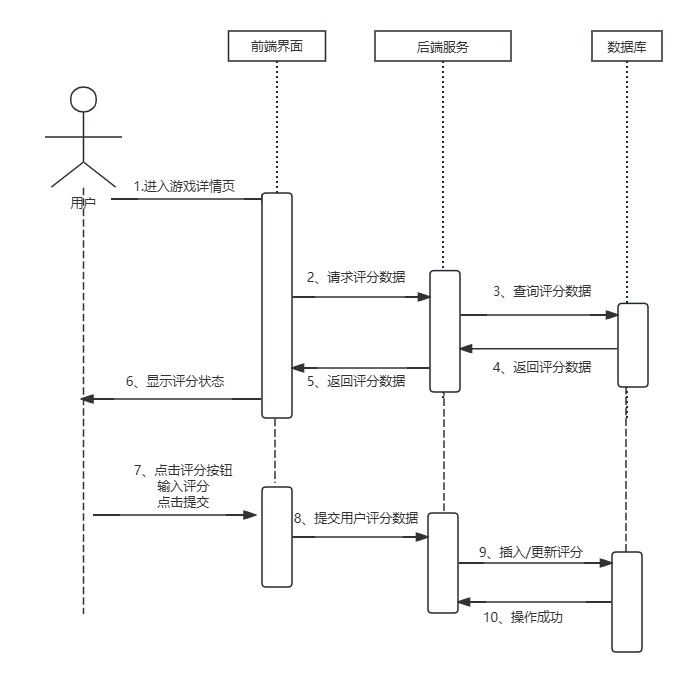
\includegraphics[width=0.7\textwidth]{yongli6.jpg}
  \caption{游戏评分主要流程请求/响应时序图}
\end{figure}
用例文档:

\begin{tabular}{|c|c|}
  \hline
  用例名称& 游戏评分\\
  \hline
  用例编号 & USE-CASE-6\\
  \hline
  行为角色 & 普通用户\\
  \hline
  简要说明 & 用户应能使用游戏评分系统\\
  \hline
  优先级 & 低\\
  \hline
  前置条件 & 已登录\\
  \hline
  后置条件 & 弹窗显示评分成功\\
  \hline
  流程 & 1、在游戏浏览界面同时显示游戏评分\\
      & 2、进入某个游戏界面\\
      &  3、点击游戏评分按钮\\
      &  4、输入评分\\
      &  5、点击提交\\
  \hline
  异常处理 & 无\\
  \hline
  备注 & 需要检测评分合法性(1-5整数)\\
  \hline
\end{tabular}

\subsubsection{游戏评论区}
支持登录用户在游戏评论区内进行交流,包括:查看评论(显示评论时间),
回复评论(响应地给被回复的用户一个通知),删除自己的评论。

主要流程请求/响应时序图:
\begin{figure}[ht]
  \centering
  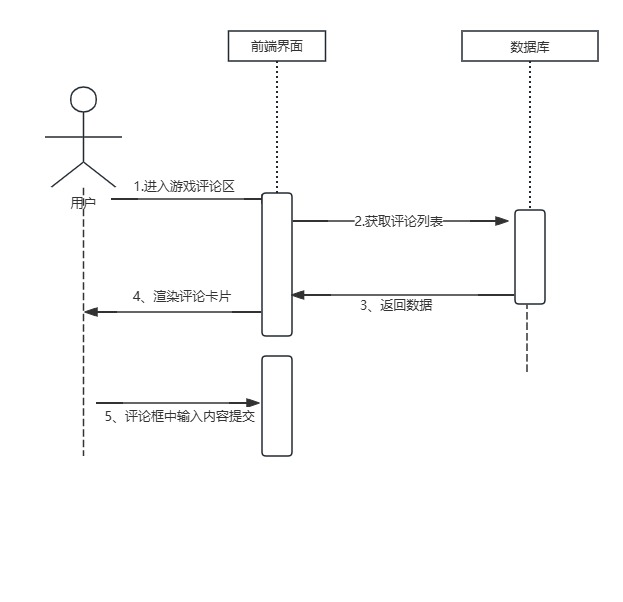
\includegraphics[width=0.7\textwidth]{yongli7.jpg}
  \caption{游戏评论区主要流程请求/响应时序图}
\end{figure}
用例文档:

\begin{tabular}{|c|c|}
  \hline
  用例名称& 游戏评论区\\
  \hline
  用例编号 & USE-CASE-7\\
  \hline
  行为角色 & 玩家\\
  \hline
  简要说明 & 用户应能使用游戏评论区交流\\
  \hline
  优先级 & 低\\
  \hline
  前置条件 & 已登录\\
  \hline
  后置条件 & 评论发表后显示在评论区,被回复后给出用户提醒\\
  \hline
  流程 & 1、进入游戏评论区\\
      &  2、查看评论\\
      &  3、点击希望恢复的评论旁的回复按钮\\
      &  4、在给出的文字编辑框中写下评论\\
      &  5、点击发表评论\\
  \hline
  异常处理 & 无\\
  \hline
  备注 & 发表的评论还应可以撤回,被回复的评论者也应有消息的提醒\\
       & 评论还需有内容不能为空,敏感词检测的检查机制\\
  \hline
\end{tabular}

\subsubsection{收藏游戏}
支持登录用户对自己喜欢的游戏进行收藏以方便用户之后的体验

主要流程请求/响应时序图:
\begin{figure}[ht]
  \centering
  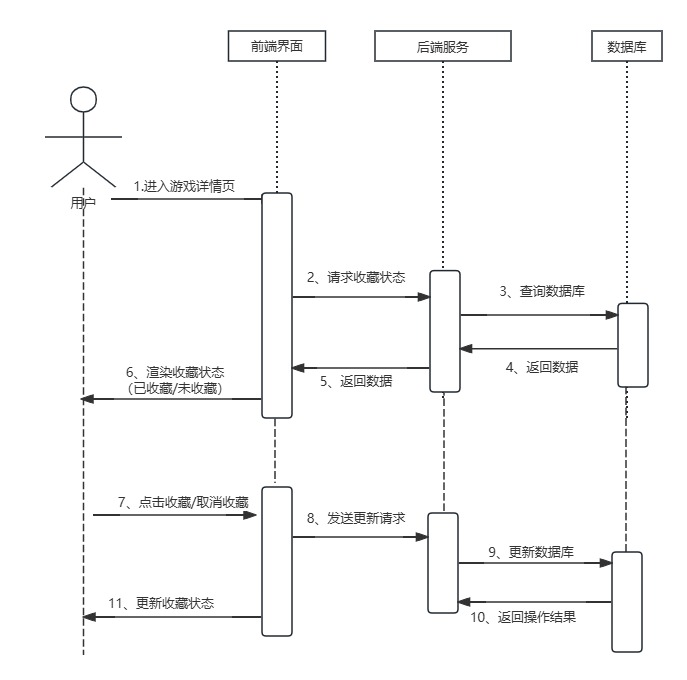
\includegraphics[width=0.7\textwidth]{yongli8.jpg}
  \caption{收藏游戏主要流程请求/响应时序图}
\end{figure}
用例文档:

\begin{tabular}{|c|c|}
  \hline
  用例名称& 收藏游戏\\
  \hline
  用例编号 & USE-CASE-8\\
  \hline
  行为角色 & 普通用户\\
  \hline
  简要说明 & 用户应能使收藏游戏\\
  \hline
  优先级 & 中\\
  \hline
  前置条件 & 已登录\\
  \hline
  后置条件 & 通过我的收藏快速找到已收藏的游戏\\
  \hline
  流程 & 1、进入某个游戏界面\\
      &  2、点击收藏按钮\\
  \hline
  异常处理 & 无\\
  \hline
  备注 & 用户还应可以管理自己的收藏,取消已收藏的游戏\\
  \hline
\end{tabular}

\subsubsection{上传游戏}
支持游戏创作者上传自己的作品以供平台用户游玩。
所需上传的包含游戏包,同时填写元数据:标题、描述、分类标签、缩略图等展示给玩家的数据,方便玩家了解游戏

主要流程请求/响应时序图:
\begin{figure}[ht]
  \centering
  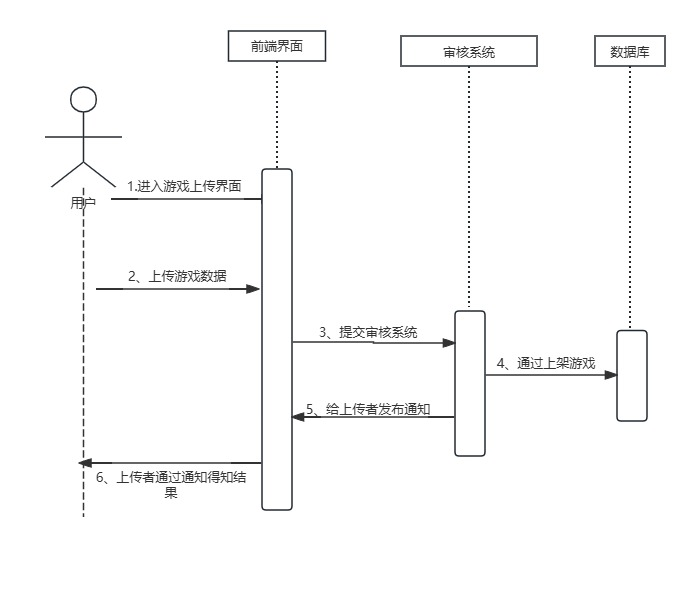
\includegraphics[width=0.7\textwidth]{yongli9.jpg}
  \caption{上传游戏主要流程请求/响应时序图}
\end{figure}
用例文档:

\begin{tabular}{|c|c|}
  \hline
  用例名称& 上传游戏\\
  \hline
  用例编号 & USE-CASE-9\\
  \hline
  行为角色 & 普通用户\\
  \hline
  简要说明 & 游戏创作者应能上传自己的作品\\
  \hline
  优先级 & 高\\
  \hline
  前置条件 & 已登录\\
  \hline
  后置条件 & 游戏在平台得到投放\\
  \hline
  流程 & 1、进入上传界面\\
      &  2、上传游戏包,设置游戏信息\\
      &  3、点击上传按钮\\
      &  4、等待管理员审核\\
      &  5、审核通过后游戏在平台得到投放\\
      &  4、审核失败后得到原因\\
  \hline
  异常处理 & 无\\
  \hline
  备注 & 无\\
  \hline
\end{tabular}

\subsubsection{管理上传的游戏}
支持游戏创作者管理自己已经上传的游戏,包括游戏包,标题、描述、分类标签、缩略图等游戏数据
的修改,已经主动下架自己的游戏;同时支持平台管理员下架游戏。

主要流程请求/响应时序图:
\begin{figure}[ht]
  \centering
  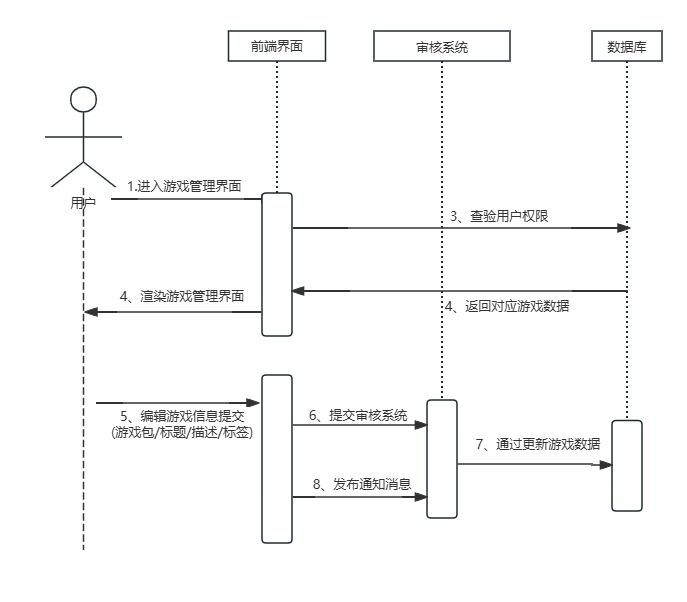
\includegraphics[width=0.7\textwidth]{yongli10.jpg}
  \caption{管理上传的游戏主要流程请求/响应时序图}
\end{figure}
用例文档:

\begin{tabular}{|c|c|}
  \hline
  用例名称& 管理游戏\\
  \hline
  用例编号 & USE-CASE-10\\
  \hline
  行为角色 & 普通用户,平台管理员\\
  \hline
  简要说明 & 游戏创作者应能管理上传的作品\\
  \hline
  优先级 & 高\\
  \hline
  前置条件 & 已登录\\
  \hline
  后置条件 & 游戏在平台得到更新/下架\\
  \hline
  流程 & 1、点击进入我的上传界面\\
      &  2、点击进入想更新的游戏的对应界面\\
      &  3、修改游戏信息\\
      &  4、点击提交\\
      &  5、等待管理员审核\\
  \hline
  异常处理 & 无\\
  \hline
  备注 & 游戏创作者下架游戏的请求应不需要审核,\\
       & 平台管理员应具有下架游戏的权利以管理游戏\\
  \hline
\end{tabular}

\subsubsection{审核游戏}
游戏的上传与更新都需要管理员审核通过,以此保证平台内容的合理性;
审核通过的内容才能在平台得到投放

主要流程请求/响应时序图:
\begin{figure}[ht]
  \centering
  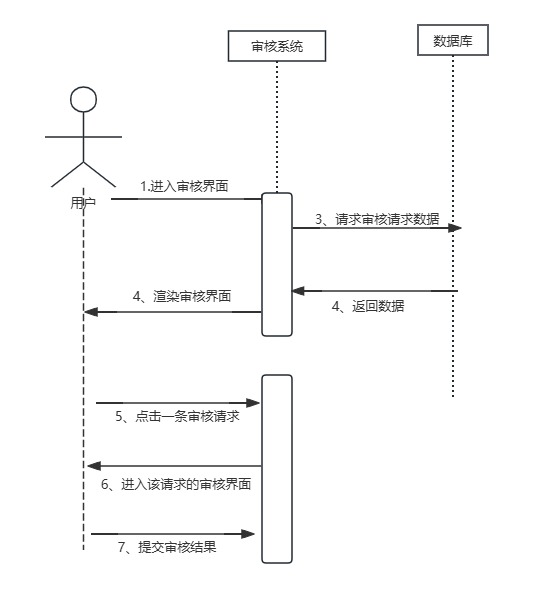
\includegraphics[width=0.7\textwidth]{yongli11.jpg}
  \caption{审核游戏主要流程请求/响应时序图}
\end{figure}
用例文档:

\begin{tabular}{|c|c|}
  \hline
  用例名称& 审核游戏\\
  \hline
  用例编号 & USE-CASE-11\\
  \hline
  行为角色 & 平台管理员\\
  \hline
  简要说明 & 内容需要审核\\
  \hline
  优先级 & 高\\
  \hline
  前置条件 & 已登录\\
  \hline
  后置条件 & 审核通过后游戏在平台得到投放\\
  \hline
  流程 & 1、点击进入审核界面\\
      &  2、点击进入想处理的请求的对应界面\\
      &  3、得到信息\\
      &  4、判断是否通过\\
      &  5、通过点击通过按钮,否则给出驳回原因\\
  \hline
  异常处理 & 无\\
  \hline
  备注 & 无\\
\end{tabular}

\subsubsection{维护游戏分类标签}
游戏分类标签由平台给出,给予管理员管理游戏分类标签的权力
以维护游戏分类标签

主要流程请求/响应时序图:
\begin{figure}[ht]
  \centering
  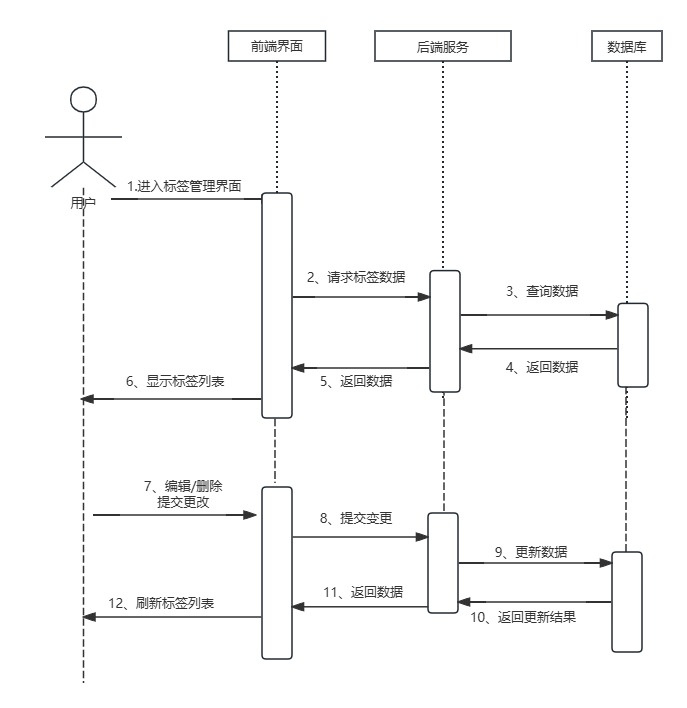
\includegraphics[width=0.7\textwidth]{yongli12.jpg}
  \caption{维护游戏分类标签主要流程请求/响应时序图}
\end{figure}
用例文档:

\begin{tabular}{|c|c|}
  \hline
  用例名称& 维护游戏分类标签\\
  \hline
  用例编号 & USE-CASE-12\\
  \hline
  行为角色 & 平台管理员\\
  \hline
  简要说明 & 游戏分类标签需要维护\\
  \hline
  优先级 & 低\\
  \hline
  前置条件 & 已登录\\
  \hline
  后置条件 & 游戏标签在平台得到修改\\
  \hline
  流程 & 1、点击进入游戏标签管理界面\\
      &  2、点击修改/增加\\
      &  3、修改:点击想修改的标签,给出修改后的该标签\\
      &  4、增加:输入想增加的标签\\
      &  5、点击确认\\
  \hline
  异常处理 &  输入已存在标签名时显示标签以重复以规避重复标签\\
  \hline
  备注 & 无\\
  \hline
\end{tabular}

\section{类图与 CRC 模型}
\subsection{类图}
% 在这里添加类图的内容
\begin{figure}[H]
  \centering
  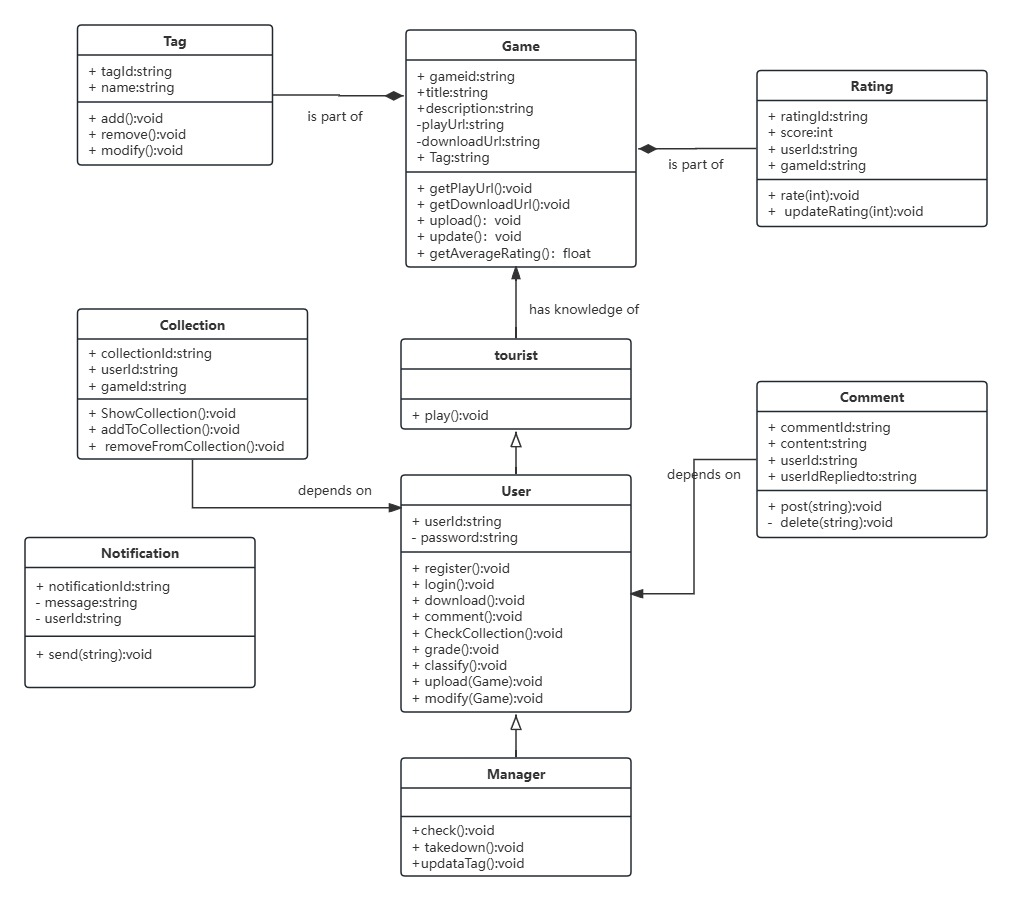
\includegraphics[width=1\textwidth]{lei.jpg}
  \caption{类图}
\end{figure}
\subsection{CRC 模型}

\subsubsection{tourist}
\begin{tabular}{|l|l|}
  \hline
  \multicolumn{2}{|l|}{类名:tourist} \\
  \hline
  \multicolumn{2}{|l|}{编号:CLASS-1} \\
  \hline
  \multicolumn{2}{|l|}{描述:使用这个系统的游客,仅有浏览与在线游玩的权限} \\
  \hline
  功能 & 合作类 \\
  \hline
  浏览 & Game,Comment\\
  \hline
  在线游玩 & Game\\
  \hline
  \end{tabular}

\subsubsection{User}
\begin{tabular}{|l|l|}
  \hline
  \multicolumn{2}{|l|}{类名:User} \\
  \hline
  \multicolumn{2}{|l|}{编号:CLASS-2} \\
  \hline
  \multicolumn{2}{|l|}{描述:使用这个系统的注册角色,包括普通用户,管理员,继承于tourist类} \\
  \hline
  功能 & 合作类 \\
  \hline
  登录进入系统 & \\
  \hline
  登出系统 & \\
  \hline
  在线游玩 & Game \\
  \hline
  下载游戏 & Game \\
  \hline
  收藏游戏 & Collection \\
  \hline
  交流 & Comment, Notification \\
  \hline
  分类检索游戏 & Tag,Game \\
  \hline
  评分 & Rating \\
  \hline
  上传游戏 & Game\\
  \hline
  更改游戏 & Game\\
  \hline
  \end{tabular}

\subsubsection{Manager}
\begin{tabular}{|l|l|}
  \hline
  \multicolumn{2}{|l|}{类名:Manager} \\
  \hline
  \multicolumn{2}{|l|}{编号:CLASS-3} \\
  \hline
  \multicolumn{2}{|l|}{描述:平台的管理者,继承于User类。} \\
  \hline
  功能 & 合作类 \\
  \hline
  审核游戏 & Game\\
  \hline
  管理游戏 & Game\\
  \hline
  维护游戏标签 & Tag\\
  \hline
  发送系统通知 & Notification\\
  \hline
  \end{tabular}

\subsubsection{Game}
\begin{tabular}{|l|l|}
  \hline
  \multicolumn{2}{|l|}{类名:Game} \\
  \hline
  \multicolumn{2}{|l|}{编号:CLASS-4} \\
  \hline
  \multicolumn{2}{|l|}{描述:代表平台上上传的游戏。} \\
  \hline
  功能 & 合作类 \\
  \hline
  在线加载 & \\
  \hline
  跳转下载地址 & \\
  \hline
  上传 &  \\
  \hline
  更新 &  \\
  \hline
  计算大众评分 & Rating \\
  \hline
  \end{tabular}

\subsubsection{Collection}
\begin{tabular}{|l|l|}
  \hline
  \multicolumn{2}{|l|}{类名:Collection} \\
  \hline
  \multicolumn{2}{|l|}{编号:CLASS-5} \\
  \hline
  \multicolumn{2}{|l|}{描述:代表一名用户的收藏} \\
  \hline
  功能 & 合作类 \\
  \hline
  展示收藏 &  \\
  \hline
  收藏游戏 & \\
  \hline
  从收藏中删除游戏 & \\
  \hline
  \end{tabular}

\subsubsection{Comment}
\begin{tabular}{|l|l|}
  \hline
  \multicolumn{2}{|l|}{类名:Comment} \\
  \hline
  \multicolumn{2}{|l|}{编号:CLASS-6} \\
  \hline
  \multicolumn{2}{|l|}{描述:代表一条用户的评论} \\
  \hline
  功能 & 合作类 \\
  \hline
  写评论 & \\
  \hline
  删评论 & \\
  \hline
  \end{tabular}

\subsubsection{Rating}
\begin{tabular}{|l|l|}
  \hline
  \multicolumn{2}{|l|}{类名:Rating} \\
  \hline
  \multicolumn{2}{|l|}{编号:CLASS-7} \\
  \hline
  \multicolumn{2}{|l|}{描述:代表一名用户对某一游戏的评分} \\
  \hline
  功能 & 合作类 \\
  \hline
  评分 & \\
  \hline
  更新评分 & \\
  \hline
  \end{tabular}

\subsubsection{Notification}
\begin{tabular}{|l|l|}
  \hline
  \multicolumn{2}{|l|}{类名:Notification} \\
  \hline
  \multicolumn{2}{|l|}{编号:CLASS-8} \\
  \hline
  \multicolumn{2}{|l|}{描述:代表对某用户的一条通知} \\
  \hline
  功能 & 合作类 \\
  \hline
  发送通知 & \\
  \hline
  \end{tabular}

\section{非功能性需求}
\subsection{性能需求}
% 在这里添加性能需求的内容

\begin{itemize}
    \item 系统应保证运行稳定,避免出现崩溃。
    \item 系统应该支持目前各主流浏览器的正常访问。
    \item 系统应能保证至少 100 人的并发访问。
    \item 对于用户对系统的所有操作,系统都应在 2s 以内做出应答。
    \item 系统应该能及时检测并报告各种非正常情况,如设备的通信终端连接失败,无法连接数据库服务器等,避免长时间等待。
    \item 每个页面一般情况下应在 2s 内加载完毕,高峰期应在 6s 内加载完毕。
    \item 系统保证在一周内不超过一次的维护与重启。
\end{itemize}

\subsection{安全性需求}
% 在这里添加输入要求的内容
\begin{itemize}
  \item 用于身份验证的用户名和密码应防止未经授权的用户访问系统。应构建访问控制以防止合法用户非法使用系统资源。某些敏感数据(如用户名,密码)在交换时应加密。密码在存储之前应加密。
  \item 用户在上传自己制作的h5游戏时,需要对上传文件的格式进行校验,如果文件大小超过限制,我们会回馈用户一个错误信息,并提示用户重新上传。
  \item 我们需要确保用户上传的文件能够正常打开,并且能够正常加载。
  \item 此外,系统应通过程序控制出错几率,减少系统因用户人为的错误引起的破坏。开发者应当尽量周全地考虑到各种可能发生的问题,使出错的可能降至最小。
  \item 在用户登录期间,应该防止数据库注入攻击,密码强制破解和伪造会话入侵等安全问题。
  \item 做好不同组用户之间权限的隔离。
\end{itemize}

\subsection{可视化需求}
% 在这里添加可视化需求的内容
\begin{itemize}
  \item 界面设计需简洁,用户体验良好。
  \item 用户提交游戏文件后,需要有相应的反馈,如上传成功,上传失败,上传进度等。
  \item 用户下载游戏文件时,需要有相应的反馈,如下载成功,下载失败,下载进度等。
  \item 平台有人提交新游戏时,需要用比较醒目的方式提醒管理员及时审核。
  \item 管理员审核通过后,制作者可以看到审核通过的通知。
  \item 新游戏上架后,向所有用户推送这个游戏的信息。
\end{itemize}

\subsection{可维护性需求}
\begin{itemize}
  \item 实现高内聚、低耦合的系统模块划分,充分考虑模块内部结构的紧密性以及模块间的独立性。
  \item 构建完备、清晰、可读的文档:维护一个好的文档结构,便于维护和查阅,同时保持文档的简明性和书写风格的一致性。
  \item 良好的编程风格:程序内部应有详细的注释和统一的编程格式,结构清晰、注释明确,使调试、测试人员能快速定位各种错误。
\end{itemize}

\section{数据流图}

以下是详细的数据流图,比较详细地展示了系统的数据流向。

\begin{figure}[H]
  \centering
  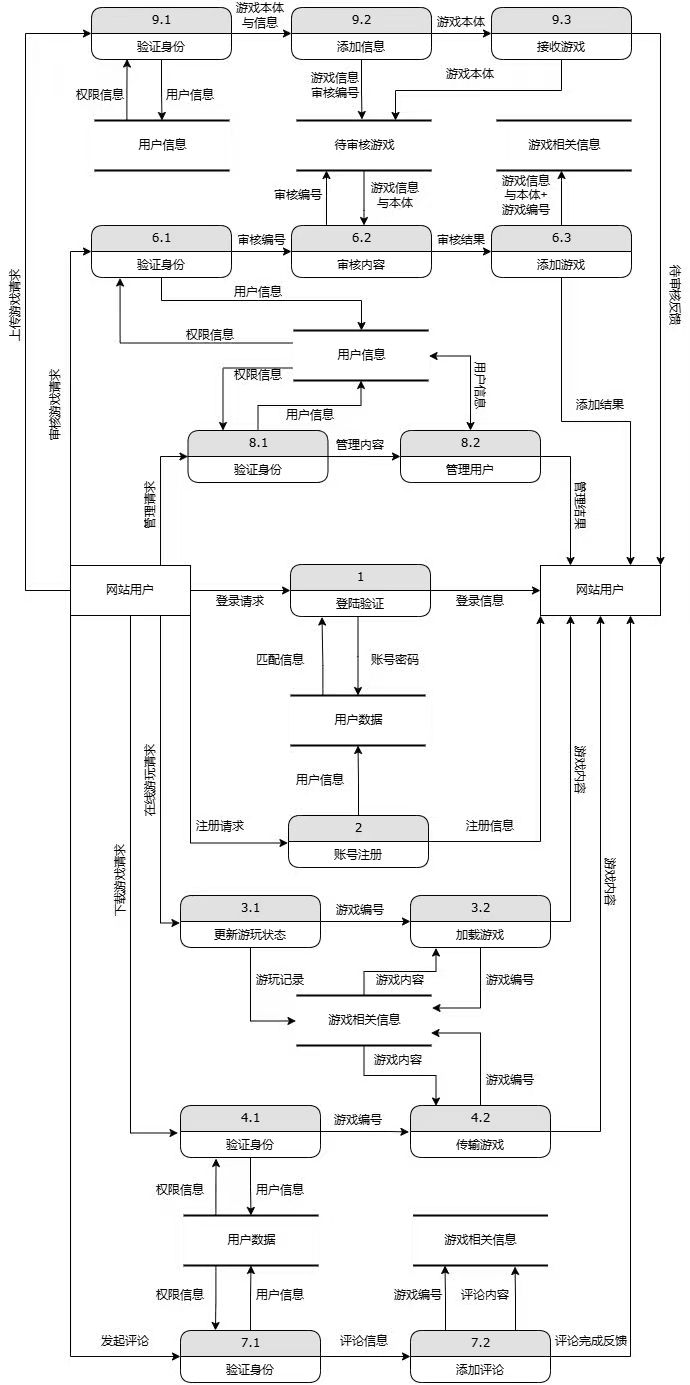
\includegraphics[width=0.6\textwidth]{dataflow.jpg}
  \caption{数据流图}
\end{figure}

\section{验收准则}
\subsection{功能要求}
% 在这里添加功能要求的内容
本系统需要完成第三节所列出的所有功能,并且通过相应的标准测试。为了保证我们试验的可靠性,我们需要招募志愿者按照他们日常游戏习惯使用我们的产品,测试产品功能。

\subsection{存储要求}
% 在这里添加存储要求的内容
由于网站里用户上传和分享的游戏数据主要是以数据库文件的形式进行存储。根据我们预估的游戏量和游戏文件的大小,我们需要确保服务器至少有1TB的存储空间。
\subsection{维护要求}
% 在这里添加维护要求的内容
系统开发的过程中程序员必须将记录开发日志,统一开发环境,时刻对源代码进行维护与管理,保证问题可被追踪。另外,软件开发团队需要进行严谨的版本控制,确保开发过程中的软件更新在认为可控的范围之内。
\section{UI 原型}

由于方案可能变化,例如登录采取第三方登录,所以我们只提供一个简单的原型,以供参考。

\subsection{登录/注册界面}
% 在这里添加登录界面的内容

\begin{figure}[htbp]
  \centering
  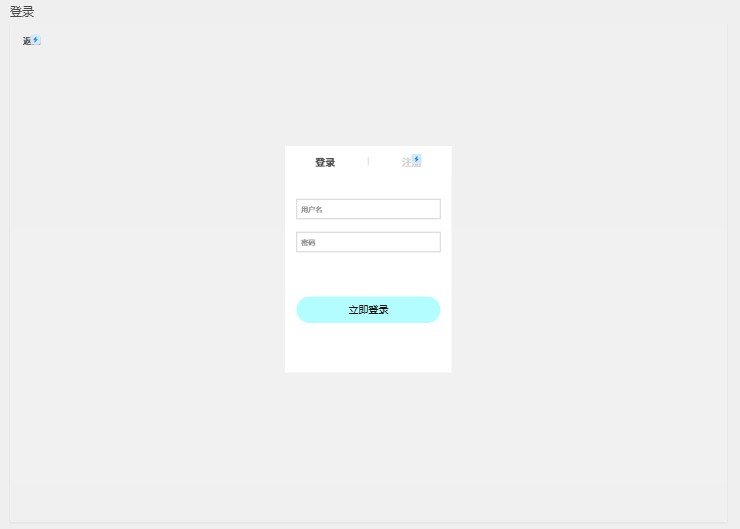
\includegraphics[width=0.55\textwidth]{login.jpg}
  \caption{登录界面}
\end{figure}

\subsection{游戏浏览界面}

\begin{figure}[H]
  \centering
  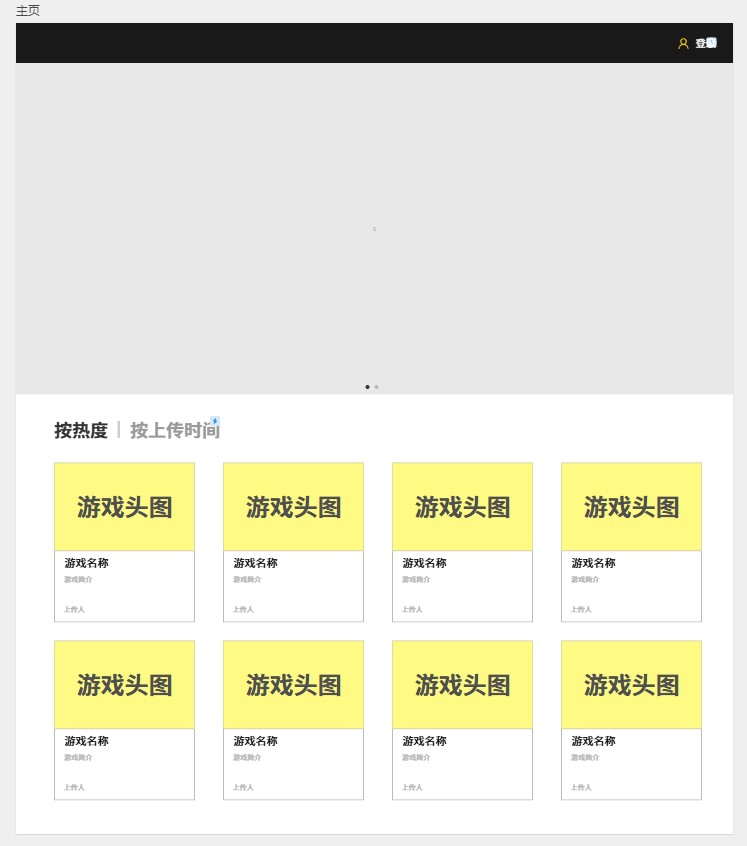
\includegraphics[width=0.55\textwidth]{main.jpg}
  \caption{游戏浏览界面}
\end{figure}

\subsection{管理员审核界面}

\begin{figure}[H]
  \centering
  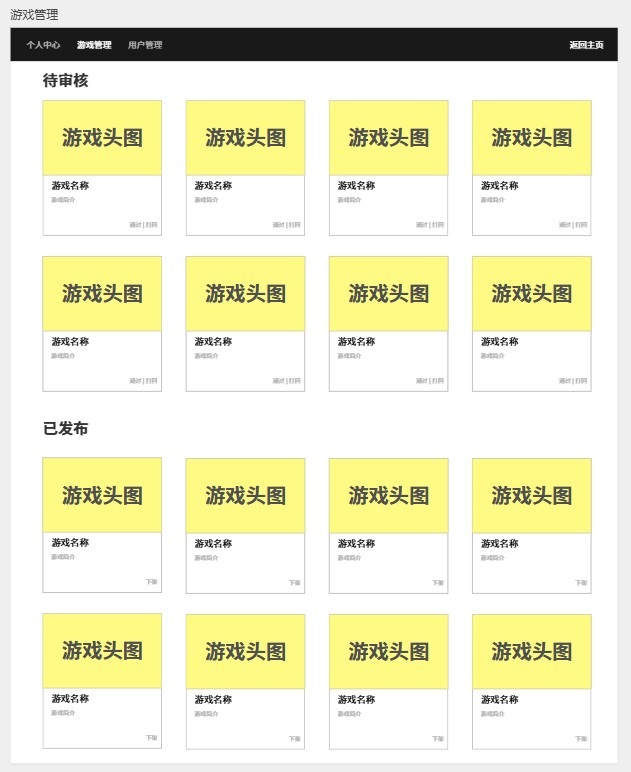
\includegraphics[width=0.5\textwidth]{admin_game.jpg}
  \caption{上传游戏审核界面}
\end{figure}

\begin{figure}[H]
  \centering
  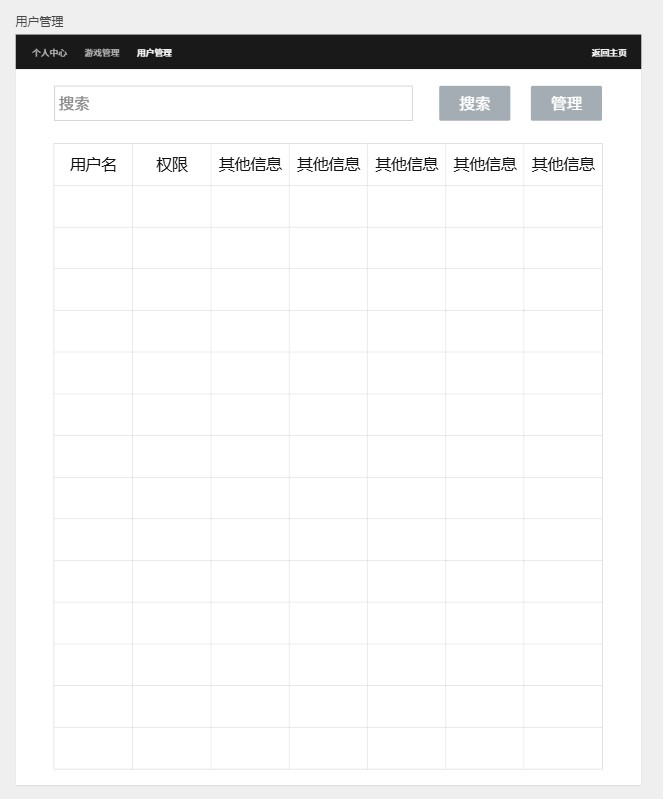
\includegraphics[width=0.5\textwidth]{admin_user.jpg}
  \caption{所有用户管理界面}
\end{figure}


\end{document}